% ****** Start of file apssamp.tex ******
%
%   This file is part of the APS files in the REVTeX 4.1 distribution.
%   Version 4.1r of REVTeX, August 2010
%
%   Copyright (c) 2009, 2010 The American Physical Society.
% 
%   See the REVTeX 4 README file for restrictions and more information.
%
% TeX'ing this file requires that you have AMS-LaTeX 2.0 installed
% as well as the rest of the prerequisites for REVTeX 4.1
%
% See the REVTeX 4 README file
% It also requires running BibTeX. The commands are as follows:
%
%  1)  latex apssamp.tex
%  2)  bibtex apssamp
%  3)  latex apssamp.tex
%  4)  latex apssamp.tex
%
\documentclass[%
reprint,
superscriptaddress,
%groupedaddress,
%unsortedaddress,
%runinaddress,
%frontmatterverbose, 
% preprint,
%showpacs,preprintnumbers,
%nofootinbib,
%nobibnotes,
%bibnotes,
amsmath,amssymb,
aps,
prl,
%pra,
% prb,
%rmp,
%prstab,
%prstper,
%floatfix,
]{revtex4-1}

\usepackage{array}
\usepackage{graphicx}% Include figure files
\usepackage{dcolumn}% Align table columns on decimal point
\usepackage{bm}% bold math
\usepackage{amsmath}
%\usepackage{hyperref}% add hypertext capabilities
%\usepackage[mathlines]{lineno}% Enable numbering of text and display math
%\linenumbers\relax % Commence numbering lines

%\usepackage[showframe,%Uncomment any one of the following lines to test 
%%scale=0.7, marginratio={1:1, 2:3}, ignoreall,% default settings
%%text={7in,10in},centering,
%%margin=1.5in,
%%total={6.5in,8.75in}, top=1.2in, left=0.9in, includefoot,
%%height=10in,a5paper,hmargin={3cm,0.8in},
%]{geometry}

% % https://tex.stackexchange.com/questions/231191/algorithm-in-revtex4-1
\usepackage{algorithm}
\usepackage{algpseudocode}


\begin{document}

\title{Fast Learning of Atomistic Rare Events: An On-the-Fly Method for Constructing Interpretable Force Fields with Gaussian Processes}

\author{Jonathan Vandermause}
\affiliation{Department of Physics, Harvard University, Cambridge, MA 02138, USA}
\affiliation{John A. Paulson School of Engineering and Applied
Sciences, Harvard University, Cambridge, MA 02138, USA}

\author{Steven B. Torrisi}
\affiliation{Department of Physics, Harvard University, Cambridge, MA 02138, USA}

\author{Simon Batzner}
\affiliation{John A. Paulson School of Engineering and Applied
Sciences, Harvard University, Cambridge, MA 02138, USA}
\affiliation{Center for Computational Engineering, Massachusetts Institute of Technology, Cambridge, MA 02139, USA}

\author{Boris Kozinsky}
\affiliation{John A. Paulson School of Engineering and Applied
Sciences, Harvard University, Cambridge, MA 02138, USA}


\date{\today}

\begin{abstract}
  Machine learning provides a path toward fast, accurate, and large-scale materials simulation, promising to combine the accuracy of \textit{ab initio} methods with the computational efficiency of classical potentials. However, training current state-of-the-art models often requires databases of first principles calculations containing thousands of structures. We present an on-the-fly Bayesian inference scheme for automating and accelerating the construction of interatomic force fields in a single molecular dynamics simulation. Gaussian process regression is coupled to a first principles DFT code to learn two- and three-body force fields on-the-fly with minimal training data. The resulting force field is easily extended to structures outside the training set and compares favorably to state-of-the-art classical and machine learned potentials.
\end{abstract}

\maketitle
Recent machine learning (ML) approaches to modelling the Born-Oppenheimer potential energy surface (PES) have been shown to approach first principles accuracy in a number of molecular and solid-state systems \cite{behler2011neural, deringer2017machine, chmiela2017machine, schutt2017schnet}. However, most ML potentials return point estimates of the quantities of interest (typically energies, forces, and stress) rather than a predictive distribution that reflects model uncertainty. Without knowledge of the highest uncertainty atomic environments, a laborious fitting procedure is required, in which thousands of reference structures are selected \textit{ad hoc} from a database of first principles calculations. At test time, lack of predictive uncertainty makes it difficult to determine when the fitted model is far from the training set, leading to unreliable results and making the model difficult to update in the presence of new data.

Here, we show that on-the-fly Gaussian process (GP) regression can accelerate the training of high-quality force fields by providing accurate estimates of model error. By combining GP regression and density functional theory (DFT) in a single molecular dynamics engine and adding only the highest uncertainty atoms to the training set, it is shown that an accurate force field can be obtained with fewer than $100$ DFT calls. Moreover, we demonstrate that the model can be flexibly updated when the system is steered away from previous training data. Such a reduction in the computational cost of training and updating potentials promises to extend ML modelling to a wider class of materials than has been possible to date. The method is shown to be well-suited to rapid crystal melts and rare diffusive events, and so we call our method FLARE: Fast Learning of Atomistic Rare Events, and make the software freely available online \cite{flare}.

The key contribution of this work is the development of a fully interpretable low-dimensional regression model of the PES that provides trustworthy estimates of model uncertainty. Typical ML schemes for modelling the PES involve regression over a high-dimensional descriptor space chosen either on physical grounds \cite{behler2011atom, bartok2013representing} or learned directly from \textit{ab initio} data \cite{schutt2017schnet, zhang2018end}. These approaches require building highly flexible models with many physically uninterpretable parameters, complicating the task of inferring a posterior distribution over possible models. We instead bypass the need for a high dimensional descriptor by imposing a physical prior that constrains the model to interactions involving two and three atoms. Because the two- and three-dimensional descriptor space of our models can be sampled with a small amount of training data, our method avoids sparsification, a procedure that is used in Gaussian approximation potentials to make inference tractable with many-body descriptors like SOAP \cite{bartok2010gaussian, bartok2013representing, bartok2015gaussian} but that is known to degrade the quality of GP variance estimates \cite{rasmussen2003gaussian}. This simplifies the learning task, making it possible to tune model hyperparameters in a data-driven fashion and derive uncertainty estimates of predictions. We show that these well-calibrated hyperparameters and uncertainty estimates make possible a practical uncertainty-driven scheme for selecting training points ``on-the-fly'', allowing an accurate potential to be learned with a minimal number of first principles calculations.

\begin{figure*}
	\centering
	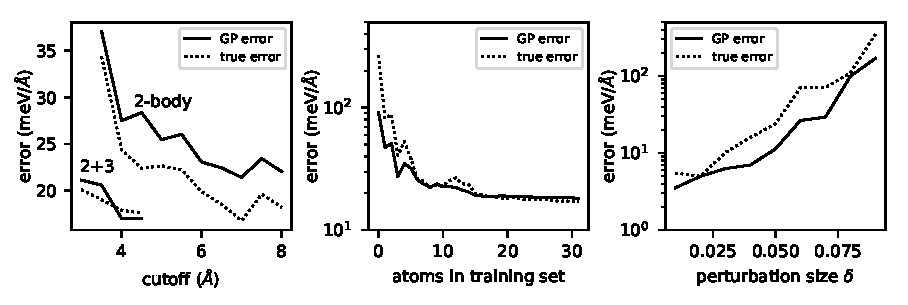
\includegraphics[width=7in]{calibrate.pdf}
	\caption{Correlation of Gaussian process noise $\sigma_n$ and predictive variance $\mathcal{V}$ with the root mean square error on independent test structures. (a) The optimized noise parameter $\sigma_n$ (solid) and root mean squared error (dotted) as a function of the cutoff radius $r_{\text{cut}}$ of the atomic environment. (b) Combined model error $\sqrt{\sigma_n^2 + \bar{\mathcal{V}}}$ as a function of the number of training atoms. (c) Mean predictive variance $\bar{V}$ (solid) and RMSE (dotted) on test structures with atomic coordinates perturbed from $\delta = 1\%$ to $9\%$ of the lattice parameter.}
\end{figure*}

To reason about model uncertainty, we use \textit{ab initio} force data to construct GP models, which provide an established and principled Bayesian scheme for estimating model uncertainty \cite{rasmussen2003gaussian}. The training database of the GP is populated with individual atomic environments by expressing the total energy of the system as a sum over two- and three-body terms,
\begin{equation}
E = \sum_{ij} \varepsilon_{ij} + \sum_{ijk} \varepsilon_{ijk},
\label{en_mod}
\end{equation}
where the sums range over all unique pairs and triplets of atoms that contain at least one atom from the unfolded primary cell. In practice, the sums are truncated by considering local atom-centered environments $\rho$ surrounding each atom in the primary cell and neglecting contributions from atoms beyond a chosen cutoff distance $r_{\text{cut}}$ from the central atom. As in \cite{glielmo2018efficient}, the covariance between bond and triplet energies is defined by a kernel that directly compares interatomic distances, so that the local energy kernel between two environments $\rho_1, \rho_2$ takes the form
\begin{equation}
k(\rho_1, \rho_2) = \frac{1}{4} \sum\limits_{\substack{i\in\rho_1 \\ j\in\rho_2}}k_2(r_i, r_j) + \frac{1}{9} \sum\limits_{\substack{i_1, i_2 \in \rho_1 \\ j_1, j_2 \in \rho_2}} k_3(\vec{d}_{i_1, i_2}, \vec{d}_{j_1, j_2}),
\end{equation}
where $r_i$ is the distance from atom $i$ to the central atom of atomic environment $\rho_1$, and $\vec{d}_{i_1, i_2} = (r_{i_1}, r_{i_2}, r_{i_1, i_2})$ is a vector of the three interatomic distances of atoms $i_1, i_2$, and the central atom of environment $\rho_1$. The fractional factors account for double- and triple-counting of bonds and triplets when computing the total energy. The resulting force kernel is obtained by differentiating this expression with respect to the Cartesian coordinates $\xi, \chi$ of the central atoms of $\rho_1$ and $\rho_2$,
\begin{equation}
k_{\xi,\chi}(\rho_1, \rho_2) = \frac{\partial^2 k(\rho_1, \rho_2)}{\partial \vec{r}_{1\xi} \partial \vec{r}_{2\chi}},
\end{equation}
giving a fully covariant and energy conserving model \cite{glielmo2017accurate, glielmo2018efficient, chmiela2017machine}.

For the bond and triplet kernels, we choose a squared exponential kernel multiplied by a smooth quadratic cutoff function that ensures the potential is continuous as atoms enter and exit the cutoff sphere,
\begin{equation}
k_{(2, 3)}(\vec{d}_1, \vec{d}_2) = \sigma_{(2, 3)}^2 \exp\left(- \frac{(\vec{d}_1 - \vec{d}_2)^2}{2 \ell_{(2,3)}^2} \right) f_{\text{cut}}(\vec{d}_1, \vec{d}_2).
\end{equation}
$\sigma_{(2, 3)}$ is related to the maximum uncertainty of points far from the training set and $\ell_{(2 ,3)}$ sets the length scale of the two- and three-body contributions. The kernel is summed over all permutations of the elements of the second descriptor vector in order to guarantee permutational invariance of the resulting force model. The force $\vec{f}_i$ on each atom $i$ and its corresponding predictive variance $\mathcal{V}[\vec{f}_i]$ are computed using the standard GP relations \cite{rasmussen2003gaussian},
\begin{equation}
	\begin{split}
f_{i\xi} &= \vec{k}^{T} \left(K + \sigma_n^2 I \right)^{-1} \vec{y} \\
\mathcal{V}[f_{i\xi}] &= k(\rho_i, \rho_i) - \vec{k}^{T} \left(K + \sigma_n^2 I \right)^{-1} \vec{k},
	\end{split}
\end{equation}
where $\vec{k}$ is the appropriate vector of force kernels between $\rho_i$ and the atomic environments in the training set, $K$ is covariance matrix $K_{mn} = k(\rho_m, \rho_n)$ of the training points, $\vec{y}$ is the vector of training force labels, and $\sigma_n$ is a hyperparameter that characterizes observation noise.

To justify our on-the-fly molecular dynamics routine, we first characterize the uncertainty and noise estimates of the two- and three-body GP models and compare them against test errors on out-of-sample structures. In all models in this work, the hyperparameters $\sigma_2, \sigma_3, \ell_2, \ell_3,$ and $\sigma_n$ are optimized with the BFGS algorithm by maximizing the likelihood of the training data, which in GP regression is efficient to compute if the model is trained on fewer than $\sim 1000$ points. This data-driven approach stands in contrast to other Gaussian process models of the PES, in which hyperparameters are chosen heuristically. Remarkably, the optimized noise parameter $\sigma_n$ and the predictive variance $\mathcal{V}$ are found to provide a sensitive probe of model error. We test the relationship between internal GP error and true error by performing a set of plane-wave DFT calculations on a 32-atom supercell of FCC aluminum with atomic positions randomly perturbed from their equilibrium sites. In Fig.\ 1(a), all atomic coordinates are randomly perturbed by up to $5\%$ of the lattice parameter, which was set to the experimental value of $4.046$ \AA. Two- and two-plus-three body GP models are trained on all forces in a single structure and tested on an independently generated structure, with the cutoff radius swept from $3.5$ and $8$ \AA. For the two-plus-three body models (lower left), the 2-body cutoff was held fixed at $6$ \AA and the 3-body cutoff was swept from 3 to 4.5 \AA. The optimized noise parameter $\sigma_n$ plotted in Fig.\ 1(a) is seen to closely track the root mean squared error (RMSE) on the test structure for the range of examined cutoffs. This provides a principled tool for selecting the cutoff radius of the GP model, showing that the expected error of the model at a given cutoff can be directly estimated from the hyperparameter $\sigma_n$.

When the GP is trained on insufficient data, we find that the predictive variance $\mathcal{V}$ rises above the baseline noise level $\sigma_n$ of the model, indicating that the model requires additional training data to make accurate force estimates. The utility of the predictive variance is illustrated in Fig.\ 1(b). Using the same training and test structures as Fig.\ 1(a), a GP model is constructed by adding atoms to the training set and evaluating the RMSE and GP error after each atom is added. The average GP error $\varepsilon = \sqrt{\sigma_n^2 + \bar{\mathcal{V}}}$ is found to closely track the RMSE, where $\bar{\mathcal{V}}$ is the mean predictive variance over all atoms in the test set. We also demonstrate in Fig.\ 1(c) that the GP variance provides an indicator of model error when the model is forced to extrapolate on structures far from the training set. A model was trained on a single structure with atomic coordinates perturbed by $\delta = 5\%$ of the lattice parameter and tested on structures generated with values of $\delta$ ranging from $1$ to $9\%$. The mean variance $\bar{V}$ is seen to correlate with the true error across all values of $\delta$, motivating the use of GP variance estimates as a reliable guide for determining when the model is far from the training set.

The reliability of the internal GP error makes possible a fully on-the-fly (OTF) molecular dynamics scheme, in which DFT is called whenever the internal error of the GP model rises above an adaptive threshold based on the optimized noise parameter $\sigma_n$. An OTF molecular dynamics run takes an arbitrary structure as input and begins with an initial call to the quantum solver. An arbitrary set of atoms and forces from the resulting scf calculation are used to initialize a GP model. The MD trajectory is then generated by the current GP model, with calls to DFT made whenever the maximum error of any force component rises above the current noise parameter $\sigma_n$ of the model. This flexible threshold ensures that DFT is called only when the predictive variance of a particular force component rises above the underlying noise level $\sigma_n$ of the model. In order to eliminate redundancy from the training set, we augment the training set with only the highest uncertainty atom whenever an scf call is made. All hyperparameters, including the noise parameter $\sigma_n$, are optimized with the BFGS algorithm whenever an atom is added to the training set, allowing the error threshold to adapt to novel environments encountered during the simulation.

\begin{figure}
	\centering
	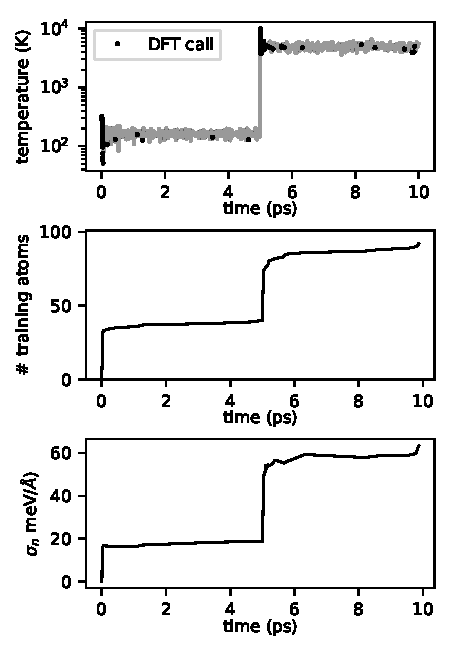
\includegraphics[width=3in]{melt.pdf}
	\caption{On-the-fly learning of a multi-phase aluminum force field. (a) Instantaneous temperature during a $10 \text{ ps}$ on-the-fly MD trajectory. The simulation begins in the FCC phase at low temperature and is melted at $5 \text{ ps}$. When the prediction error on a given force component rises above the current noise parameter $\sigma_n$ of the model, DFT is called (black dots). (b) The number of atoms in the training set throughout the simulation. A sharp increase is observed when the crystal is melted, illustrating the model's ability to adapt to the liquid phase. (c) The optimized noise parameter $\sigma_n$ and all other hyperparameters of the kernel are re-optimized whenever an atom is added to the training set. The noise level increases sharply during the melt.}
\end{figure}

The scheme is implemented by coupling the Quantum Espresso DFT code \cite{giannozzi2009quantum} to MD and GP code using the FLARE package \cite{flare}. We demonstrate this on-the-fly routine by applying it to a 32 bulk aluminum system (Fig.\ 2). The simulation begins in the FCC phase at low temperature. As shown in Fig.\ 2(a), DFT is called often at the beginning of the simulation as the GP model learns a force field suitable for FCC aluminum. After about 30 timesteps, the model needs far fewer training points, requiring fewer than 50 training atoms in the first $5 \text{ ps}$ of the simulation. To test the model's ability to flexibly adapt to changing conditions, the crystal is melted at time $t = 5 \text{ ps}$ by rescaling the velocities of the atoms. As shown in the right side of Fig.\ 2, the GP model requires a large number of DFT calls immediately after the crystal is melted, as the atomic environments in the liquid phase of aluminum are significantly different from the previous training data. As shown in Fig.\ 1(c), the noise parameter $\sigma_n$ of the model sharply increases as the system enters the liquid phase, reflecting the fact that it is more difficult to model the high temperature liquid phase, which involves more diverse atomic environments and significantly larger forces. Because the error threshold is set equal to $\sigma_n$, the threshold in the liquid phase is relaxed, and as a result the GP model requires a roughly similar number of DFT calls for both the solid and liquid phases. As shown in Fig.\ 2(b), fewer than $100$ calls are needed in total, with the majority of DFT calls made at the beginning of the simulation and during the melt.

\begin{table}
	\centering
	\begin{tabular}{c c c c} 
	 \hline
	 \hline
	 Test Set & FLARE & AGNI \cite{botu2016machine} &  EAM \cite{sheng2011highly} \\ 
	 \hline
	 FCC Solid & 32.9 & 41.2 & 46.1 \\ 
	%  300 K & & & \\
	%  500 K & & & \\
	%  700 K & & & \\
	 Liquid & 90.2 & 128.0 & 157.0 \\
	 \hline
	 \hline
	\end{tabular}
\caption{Error of FLARE models on test structures drawn from \textit{ab initio} molecular dynamics trajectories of a 2x2x2 supercell of bulk aluminum in the solid and liquid phases. Errors are reported in $\text{meV/\AA}$.}
\end{table}

The performance of the potential obtained with the OTF run in Fig.\ 2 is validated by testing the model on two independent $10 \text{ ps}$ \textit{ab initio} molecular dynamics simulations of the solid and liquid phases of aluminum, which we performed using the Quantum Espresso code. $100$ structures were sampled from the AIMD trajectories with $0.1 \text{ ps}$ spacing between structures. Force predictions on all test structures were obtained with the OTF potential of Fig.\ 2 and compared against the corresponding \textit{ab initio} values, with the mean absolute error in \text{meV/\AA} recorded in Table 1. For reference, the models are compared against a state-of-the-art aluminum EAM potential \cite{sheng2011highly} and a recent aluminum ML potential \cite{botu2016machine}. Each potential is tested on the same AIMD structures, with the FLARE potential reaching the lowest force errors for both trajectories.

Finally, we demonstrate that FLARE can be used to analyze rare-event dynamics over timescales spanning hundreds of picoseconds by studying vacancy diffusion in a 32-atom bulk aluminum system during a $1 \text{ ns}$ OTF simulation. The GP model was constructed with a two-body kernel with cutoff $r_{\text{cut}} = 5.4 \text{ \AA}$. The system is initialized by removing one atom from an equilibrium FCC structure and setting the instantaneous temperature of $1500 \text{ K}$, giving a mean temperature of $\approx 734 \text{ K}$ for the entire run. As shown in Fig.\ 3(a), most DFT calls are made early on in the simulation. After the first $\sim 400 \text{ ps}$, no additional DFT calls are required, and the model is shown to capture vacancy hopping every few hundred picoseconds. To check the accuracy of the underlying energy model of the GP, DFT energies were computed along a high symmetry transition path. The GP force predictions along the transition path were integrated to give an estimate of the energy barrier, showing close agreement to the $\textit{ab initio}$ values.

\begin{figure}
	\centering
	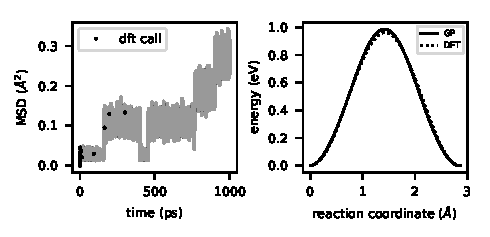
\includegraphics[width=3.41in]{vac.pdf}
	\caption{On-the-fly learning of vacancy diffusion in bulk aluminum. Left: Mean squared displacement during an OTF run of duration $1 \text{ ns}$. The majority of DFT calls occur at the beginning of the run, with no additional calls required after the first $400 \text{ ps}$. Right: the energy model of the resulting FLARE potential is tested on a high symmetry transition path, in close agreement with the \textit{ab initio} barrier.}
\end{figure}

In summary, we have presented a scheme for rapidly training GP models that provide accurate force estimates and reliable estimates of model uncertainty. The noise hyperparameter $\sigma_n$ and predictive variance $\mathcal{V}$ of the model is shown to correlate with out-of-sample error, providing a principled basis for on-the-fly molecular dynamics. The FLARE potentials described here require a small number of atomic environments to converge the model, and are therefore well-suited to settings in which large databases of \textit{ab initio} data are too expensive to compute. Our models have a simple underlying energy model described by Eq.\ (\ref{en_mod}), which can be used to map the potential to a faster regression model approaching the efficiency of a classical force field \cite{glielmo2018efficient}. This may provide a path toward potentials with the accuracy of DFT and the efficiency of a classical two-plus-three body potential, which we expect to considerably expand the range of material systems that can be accurately studied with atomistic simulation.
\bibliography{otf.bib}

\end{document}
